% Abstract + introduction draft (ARR August), v5. Benchmark name via \bench macro below.
% STYLE RULES for this paper (author preference): no semicolons, no em-dashes in prose.
%   Prefer active voice (passive only when the agent is irrelevant). Prefer simple
%   if-structures ("If X, we discard Y") over result-clause chains. Mark examples
%   explicitly ("For example", "For instance", "as in Figure 1B"), never a bare
%   "(Figure 1B)" parenthetical. Do not concatenate independent clauses with
%   ", and": split into separate sentences. No aphoristic two-fragment
%   rhetoric ("X is not the bottleneck. Y is."): state the claim in one
%   professional sentence. Do not restate in prose numbers already printed
%   in a referenced table or figure unless the sentence adds a contrast.
% Positioning (fundamental, not incremental):
%   Image-based work (RAcQUEt etc.) documents a failure of conversational HABIT:
%   the alternatives are co-present and largely perceived, models just do not mention them.
%   In video, the readings must be COMPUTED (event individuation, identity tracking,
%   memory), so the same surface behavior hides a different fault: inability, not
%   unwillingness. The benchmark + interactive protocol + scaffold are the instruments
%   that separate the two. Findings: the fault in video is inability.
\documentclass[11pt]{article}
\usepackage[review]{acl}   % ARR submission mode: anonymous + line numbers
\usepackage{times}
\usepackage{latexsym}
\usepackage[T1]{fontenc}
\usepackage[utf8]{inputenc}
\usepackage{microtype}
\usepackage{inconsolata}
\usepackage{graphicx}
\usepackage{booktabs}
\usepackage{pifont}
\usepackage{xcolor}
\newcommand{\cmark}{\ding{51}}
\newcommand{\xmark}{\ding{55}}

% Benchmark name is a macro. Rename in ONE place. Candidates (collision-checked on arXiv):
%   ReQueST = REferential QUEstions Spanning Time; also evokes clarification requests  <- current
%   DejaVQA (deja vu pun, no acronym), WhichWhen (no acronym)
%   avoid: VAGUE (taken, same subfield!), REWIND (taken in vision), TeRA, AMBER (taken)
\newcommand{\bench}{ReQueST}
\newcommand{\benchicon}{\raisebox{-0.18em}{
\includegraphics[height=1.05em]{figures/request_icon.png}}}

% Compress float/caption/section spacing so the seven main-body floats fit within
% the 8-page limit. Limitations still opens page 9.
\setlength{\textfloatsep}{3pt plus 2pt minus 2pt}
\setlength{\floatsep}{3pt plus 2pt minus 2pt}
\setlength{\intextsep}{3pt plus 2pt minus 2pt}
\setlength{\dbltextfloatsep}{4pt plus 2pt minus 2pt}
\setlength{\abovecaptionskip}{2pt}
\setlength{\belowcaptionskip}{0pt}
% allow denser float packing so a seventh float fits on the text pages
\renewcommand{\topfraction}{0.95}
\renewcommand{\bottomfraction}{0.9}
\renewcommand{\textfraction}{0.06}
\renewcommand{\floatpagefraction}{0.85}
\setcounter{topnumber}{3}
\setcounter{bottomnumber}{2}
\setcounter{totalnumber}{4}
% trim vertical space around (sub)section headings
\usepackage{float}
\usepackage{titlesec}
\titlespacing*{\section}{0pt}{3pt plus 1pt minus 1pt}{2pt}
\titlespacing*{\subsection}{0pt}{3pt plus 1pt minus 1pt}{2pt}
\titlespacing*{\paragraph}{0pt}{3pt plus 1pt minus 1pt}{1em}

\title{\benchicon{}\,\bench{}: One Question, Many Readings\\in Video Question Answering}
% Alternative titles, same register:
%  - "One Question, Many Readings: How Video-Language Models Handle Referential Ambiguity"
%  - "Answering Without Asking: Hallucinated Commitment on Ambiguous Video Questions"

\author{Anonymous ACL submission}

\begin{document}
\maketitle

\begin{abstract}
To answer a question, one must first determine what it asks. Questions about videos often admit several readings, since they may refer to multiple entities or moments. While humans respond to such referential ambiguity by seeking clarification or addressing each alternative, most video-language models commit to a single reading, a behavior we term \textit{hallucinated commitment}. We examine this failure by introducing \textbf{\bench{}}, a benchmark that pairs each question with exhaustive, human-validated readings and per-reading answers. Unlike in images, a video question's readings are distributed over time. Most models commit silently even when invited to ask. The models that do ask often answer the named reading incorrectly. Fine-tuning induces \textit{format mimicry}: models adopt the style of ambiguity-aware answers but fill them with incorrect readings. Once the validated readings are supplied, the open-weight models answer nearly perfectly, so for them the bottleneck is finding the readings, not answering them. Our results underscore the urgency of equipping models to determine what a question asks before answering it.
\end{abstract}

\begin{figure}[t]
\centering
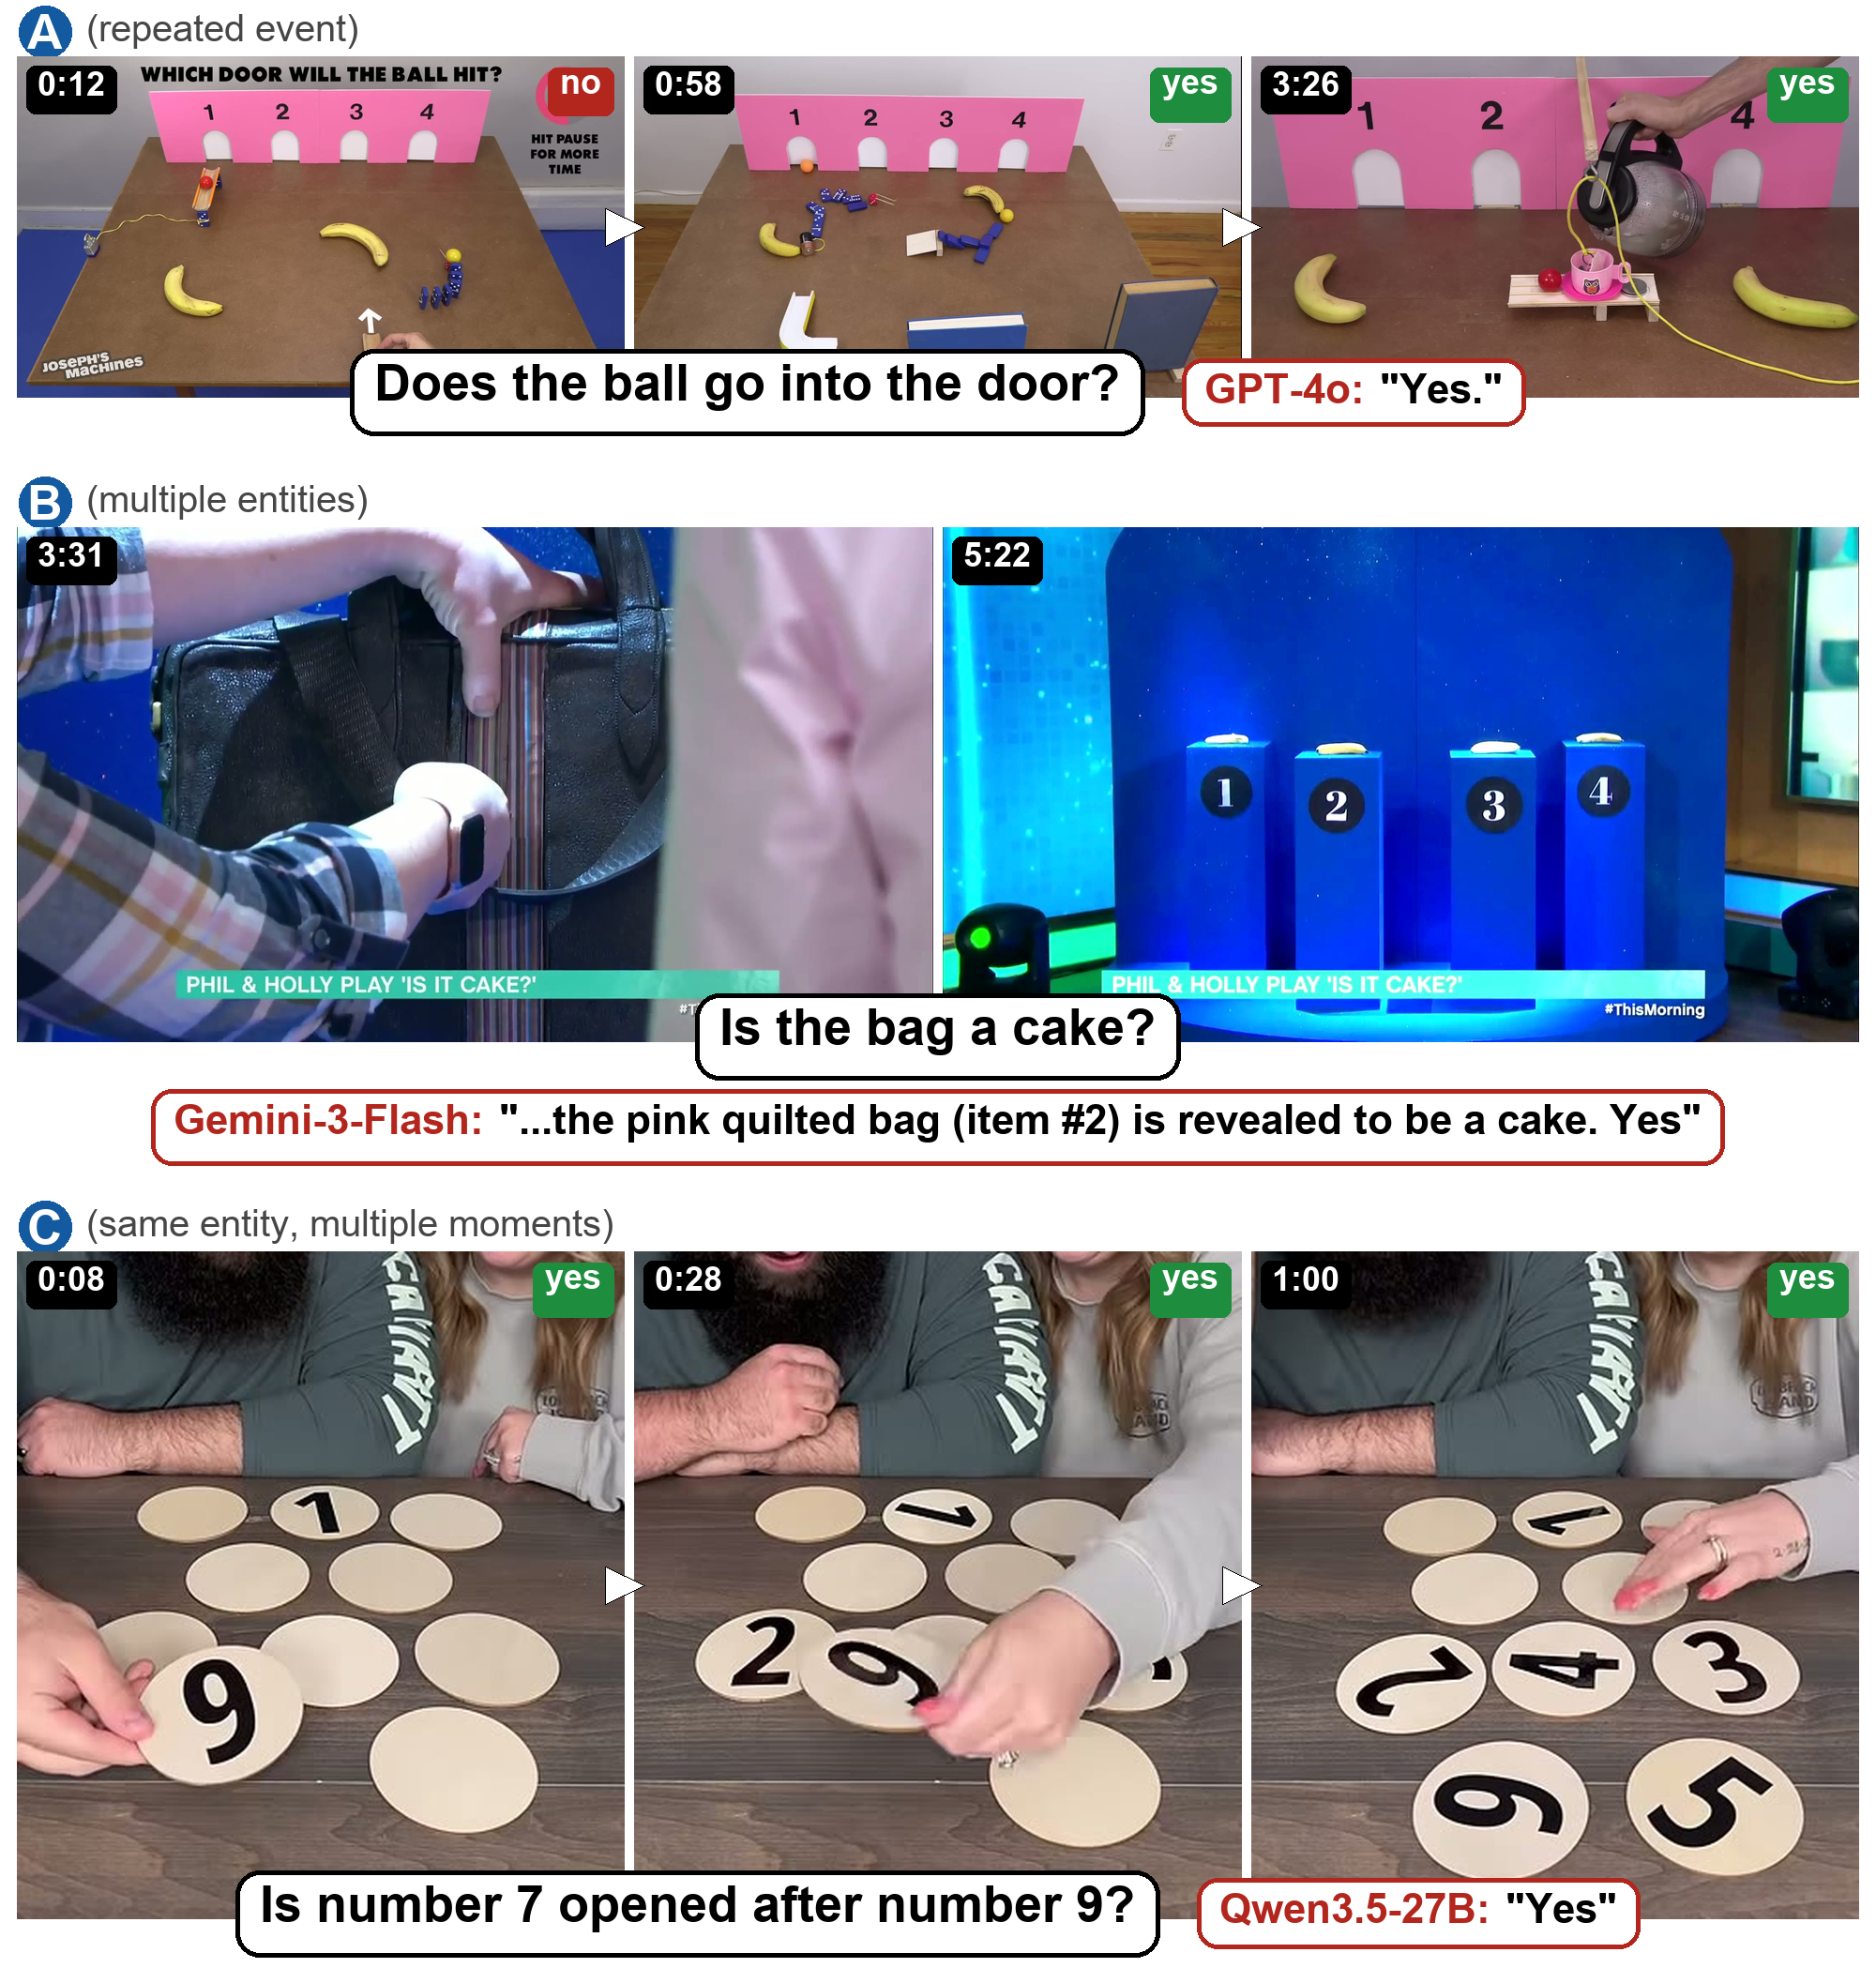
\includegraphics[width=\columnwidth]{figures/figure1.png}
\caption{Ambiguous question-video pairs from \bench{}, with the timestamps of the candidate referents and, in red, a verbatim model response to each question. \textbf{(A)} the mentioned event happens more than once, and the correct answer is no for the first attempt but yes for the later two: GPT-4o commits to a single reading. \textbf{(B)} several entities match the mentioned attribute: Gemini-3-Flash selects one of the four bags and answers for it, incorrectly. \textbf{(C)} the same entity is involved at multiple moments (here the readings happen to agree). In (A) and (C), the readings never appear together in a single frame.}
\label{fig:teaser}
\end{figure}

\section{Introduction}

Imagine watching a video of a homemade chain-reaction machine (Figure~\ref{fig:teaser}A). A friend glances over your shoulder, catches a ball rolling toward a wall of numbered doors, and asks: \textit{``Does the ball go into the door?''}. The video shows three attempts minutes apart: the first ball stops just short, the second and third roll in. You may ask which attempt your friend means, recall which attempt was on screen and answer that one, or answer for each attempt in turn.

None of these responses is unusual, since language is pervasively ambiguous and conversation repairs it routinely \citep{piantadosi2012communicative,clark1996using}. Every such repair begins by locating the candidate referents the question could pick out, each of which gives the question a distinct reading. Psycholinguistic studies show how listeners do this when the candidates are in view: they distribute their gaze across the candidates in the scene \citep{sedivy1999achieving,spivey2002eye,chambers2002circumscribing}. A viewer of a video has no single scene to scan, because ongoing activity is experienced as a sequence of episodes, segmented while watching and later retrieved from memory \citep{zacks2007event}. The readings of the friend's question belong to episodes minutes apart (Figure~\ref{fig:teaser}A) and must be recalled and compared in memory. Referential ambiguity in video is therefore largely ambiguity \textit{in time}, a dimension a single image cannot have.

Current video-language models fail to resolve this temporal ambiguity. Asked the friend's question, GPT-4o returns the complete response \textit{``Yes.''} whereas Qwen3.5 returns \textit{``No.''}, each silently selecting a different attempt from the three available (Figure~\ref{fig:teaser}A). The commitment persists with more verbose output. In Figure~\ref{fig:teaser}B, Gemini names one of four candidate bags, restricts its answer to that bag, and that answer is incorrect. We call this behavior \textit{hallucinated commitment}, by analogy to object hallucination, which invents content absent from the video \citep{rohrbach2018object}. What the model invents is not content but the uniqueness of the referent: it silently accommodates the question's presupposition that exactly one is meant \citep{lewis1979scorekeeping} instead of challenging it.

This temporal ambiguity is a specific form of referential ambiguity, previously studied in text and static images. In text, more than half of naturally occurring questions admit multiple valid answers \citep{min2020ambigqa,stengeleskin2023chicken}. In images, vision-language models describe a single salient referent \citep{testoni2025racquet} rather than request clarification \citep{jian2025clearvqa,wang2025mucar}. Because such questions admit no single correct answer, existing benchmarks provide no gold labels and instead classify the form of a response as committing, hedging, or asking. For images, this design is well motivated: the alternatives are visible and often mentioned in models' reasoning traces \citep{testoni2025racquet}, so a commitment reflects an unwillingness to report what the model has perceived. In video, where readings must be recalled rather than observed, the same commitment may instead reflect an inability to identify the readings. Separating the two requires an evaluation that accepts clarification requests and can score any reading against a gold answer. Accepting clarification means a silent commitment is no longer forced by the task. Gold scoring then tests identification.

To provide such an evaluation, we introduce \bench{}\,\benchicon{}: a benchmark of REferential QUEstions Spanning Time. \bench{} comprises 1{,}056 ambiguous questions about 80 videos, split into an \textbf{entity} subset where co-occurring entities share the mentioned attribute (Figure~\ref{fig:teaser}B) and an \textbf{event} subset where the same event or entity recurs over time (Figure~\ref{fig:teaser}A,C). Unlike image-based predecessors, \bench{} includes gold answers. Every question carries an exhaustive, human-validated list of yes-or-no readings, so a validated automatic judge can score any response strategy. A model may therefore answer for every reading, or it may ask for clarification and receive a scripted, deterministic reply naming the intended reading, which keeps the evaluation reproducible.

We assess proprietary and open-weight video-language models on \bench{}. While a human respondent would ask or answer for each reading, most models we test commit silently on the majority of questions, even when the prompt offers the option to ask. In a separate diagnostic the open-weight models answer nearly perfectly once we supply the gold readings, so for them the failure lies in finding rather than answering. As this diagnosis predicts, the event subset, whose readings must be recalled across time, proves the more difficult of the two. Commitments are systematic, favoring particular temporal positions and salient entities. The inability to find readings resists prompting, interactive clarification, fine-tuning, and reinforcement learning, which marks the problem as an open challenge. Fine-tuning fails most instructively, yielding \textit{format mimicry}, multi-reading templates filled with wrong readings, and this pattern both localizes the difficulty and charts directions for future research. These results are a warning sign for the reliability of video assistants: as footage grows longer and people or events recur, a model that commits silently may deliver confident answers to readings the user never intended.

\section{Related Work}

\paragraph{Ambiguity in language and question answering.} Ambiguity is a design feature of efficient communication rather than a defect \citep{piantadosi2012communicative}, and listeners resolve most of it incrementally from context \citep{ferreira2008ambiguity, sedivy1999achieving}. When context does not suffice, interlocutors ground the intended reading through dialogue \citep{clark1991grounding, clark1996using}. Text-only benchmarks operationalize the phenomenon as questions with several plausible answers: AmbigQA \citep{min2020ambigqa} asks models to surface all of them, and follow-up work studies when models should ask instead of answering \citep{stengeleskin2023chicken}. In these resources the ambiguity lives in world knowledge or in retrieval. \bench{} moves it into the visual referent of a fixed surface question.

\paragraph{Referential ambiguity in images.} RAcQUEt \citep{testoni2025racquet} shows that image-grounded models answer referentially ambiguous questions about one referent without acknowledging the others, a behavior the authors link to overconfidence and to social bias. ClearVQA \citep{jian2025clearvqa} trains models to ask clarifying questions on ambiguous image--question pairs, MUCAR \citep{wang2025mucar} extends the setting across languages, and earlier work probed uncertainty acknowledgment more broadly \citep{liu2023afraid, pezzelle2023dealing}. In all of these, the competing referents are co-present in a single frame, so silent commitment can persist even when every candidate is perceived. In video, the readings are distributed over time and must be computed through event individuation and identity tracking \citep{zacks2007event}, so the same surface behavior can hide a different fault. Our diagnostics separate the two, and \S\ref{sec:diagnostics} locates the video fault in computing the readings.

\paragraph{Video benchmarks and hallucination.} Standard video question-answering benchmarks such as MVBench \citep{li2024mvbench} and Video-MME \citep{fu2024videomme} assign one correct answer per question, so a model that commits to a single reading is never penalized. Video hallucination benchmarks measure fabricated content \citep{liu2025vidhalluc, choong2025vidhal}, following image-side analyses of object hallucination \citep{rohrbach2018object}; question ambiguity itself has been treated as a nuisance variable to remove \citep{bhattacharya2019why}. The failure \bench{} targets is complementary to both: nothing the model says is fabricated, and the harm lies in the $K-1$ readings it never considered.

Table~\ref{tab:comparison} summarizes the contrast with the closest resources along the axes that matter for hallucinated commitment: modality, temporal distribution of the alternatives, exhaustive gold reading lists, and an interactive protocol that lets asking pay off.

\section{\bench{}: A Benchmark for Referential Ambiguity in Video}
\label{sec:benchmark}

\subsection{Dataset Construction}
\label{sec:construction}

\bench{} pairs 80 videos with 1{,}056 referentially ambiguous yes/no questions. Each question has an exhaustive list of $K$ readings. Each reading names its referent, restates the question with that referent resolved, and specifies a gold answer. Example: in Figure~\ref{fig:teaser}A the three readings refer to the first, second, and third attempts and restate the question. The gold answer is no for the first attempt and yes for the later two.

The videos feature similar co-occurring entities or recurring events, so short questions can underdetermine a referent. A vision-language model over-generates candidate questions with proposed reading lists. We keep only candidates that meet three requirements. First, the list must include the reading a viewer would reach first. Example: in a two-round game, \textit{``the winner''} in \textit{``does the winner celebrate?''} could mean the winner of either round or the overall winner. Viewers default to the overall winner. If a candidate lists only the two round winners, it omits this default reading and we discard it. Second, the mentioned referent must have a countable set of clearly visible groundings. Example: \textit{``the person''} in a street scene full of incidental passersby admits no stable exhaustive reading list, so it offers no fair target. Third, the ambiguity must arise from video entities and events rather than from a static layout. Example: in a split-screen broadcast showing two games side by side, \textit{``does the game end in a draw?''} is ambiguous only between the left and right halves of the frame, a static layout ambiguity that a single frame already exhibits. Human annotators validate every surviving question, checking that the reading list is exhaustive and that each gold answer holds (guidelines in Appendix~A). We release a public development split of 256 questions and withhold the 800-question test split.

Questions average 6.4 tokens, so ambiguity stems from video content rather than complex phrasing. The number of readings ranges from 2 to 56 with a mean of 6.1 (Figure~\ref{fig:stats}, left). Readings are consequential rather than interchangeable: in 92.0\% of questions at least two readings have different gold answers, so resolving to the wrong reading can change the user's answer.

\begin{figure}[t]
\centering
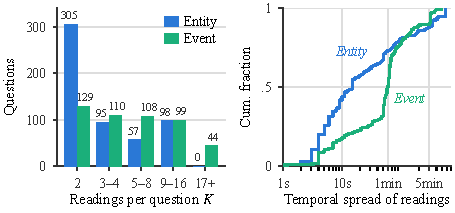
\includegraphics[width=\columnwidth]{figures/fig2_stats.pdf}
\caption{\bench{} statistics. \textbf{Left}: questions per number of readings $K$, by subset. \textbf{Right}: cumulative distribution of temporal spread, defined as the span between the earliest and latest gold evidence timestamps of a question's readings. For the event subset the median spread is one minute of footage. For a tenth of the questions it exceeds five minutes.}
\label{fig:stats}
\end{figure}

\paragraph{Large $K$.} We keep high-$K$ questions that image benchmarks exclude. RAcQUEt admits a question only when its target category has at most ten referents \citep{testoni2025racquet}. That design follows from scoring a single response, since cooperative speakers do not enumerate dozens of alternatives, so high-$K$ questions would be unfair there. Two properties make them fair here. First, they are combinatorial rather than vague: a high-$K$ case is a short question asked of footage where the same visible events recur many times. $K$ reaches 56 when a question relates two event types that recur eight and seven times, since each reading corresponds to one pair of occurrences. Validating such a list reduces to counting recurrences. Second, our protocol never requires enumeration: a clarifying question earns full credit at any $K$ (\S\ref{sec:protocol}). The scripted reply names a single intended reading, so the follow-up needs one answer, not 56. Large-$K$ questions therefore make clarification the natural strategy, which is the behavior the benchmark measures. We stratify all results by $K$ so no conclusion depends on the tail.

\paragraph{Subsets.} Following the two sources of ambiguity in Figure~\ref{fig:teaser}, \bench{} defines two subsets.\footnote{The remaining 11 questions mix both sources and are counted only in aggregate results.} In \textbf{\bench{}-Entity} (555 questions, 71 videos, mean $K$ of 4.6) several co-occurring entities match the mentioned attribute, as in Figure~\ref{fig:teaser}B, so readings are typically available within one scene and their gold evidence spans a median of 15 seconds. In \textbf{\bench{}-Event} (490 questions, 33 videos, mean $K$ of 7.9) the mentioned event or entity recurs, as in Figures~\ref{fig:teaser}A and \ref{fig:teaser}C, so readings are indexed by occurrence and separated in time with evidence that spans a median of one minute. In a tenth of questions, the earliest and latest evidence lie more than five minutes apart (Figure~\ref{fig:stats}, right). The two subsets operationalize the contrast from the introduction between readings that can be scanned within one scene and readings that must be recalled across episodes. Table~\ref{tab:comparison} situates the resource: among the benchmarks compared, \bench{} alone has readings separated in time and combines exhaustive reading lists, per-reading gold answers, and a scored clarification path.

\begin{table}[t]
\centering
\small
\setlength{\tabcolsep}{4.2pt}
\begin{tabular}{@{}lccccc@{}}
\toprule
Benchmark & Mod. & Time & Exh. & Gold & Inter. \\
\midrule
AmbigQA & text & \xmark & \cmark & \cmark & \xmark \\
Stengel-Eskin & image & \xmark & \cmark & \cmark & \xmark \\
RAcQUEt & image & \xmark & \xmark & \xmark & \xmark \\
ClearVQA & image & \xmark & \xmark & \xmark & \cmark \\
MUCAR & image & \xmark & \xmark & \xmark & \xmark \\
\midrule
\bench{} (ours) & video & \cmark & \cmark & \cmark & \cmark \\
\bottomrule
\end{tabular}
\caption{Comparison of \bench{} with ambiguity benchmarks in text \citep{min2020ambigqa}, visual QA \citep{stengeleskin2023chicken,testoni2025racquet,jian2025clearvqa}, and cross-modal resolution \citep{wang2025mucar}. \textbf{Time}: readings separated in time rather than co-present in one scene. \textbf{Exh.}: exhaustive human-validated reading lists. \textbf{Gold}: a gold answer per reading, so any response strategy is scorable. \textbf{Inter.}: a scored interactive clarification path.}
\label{tab:comparison}
\end{table}


\subsection{Interactive Protocol and Metrics}
\label{sec:protocol}

\begin{figure*}[t]
\centering
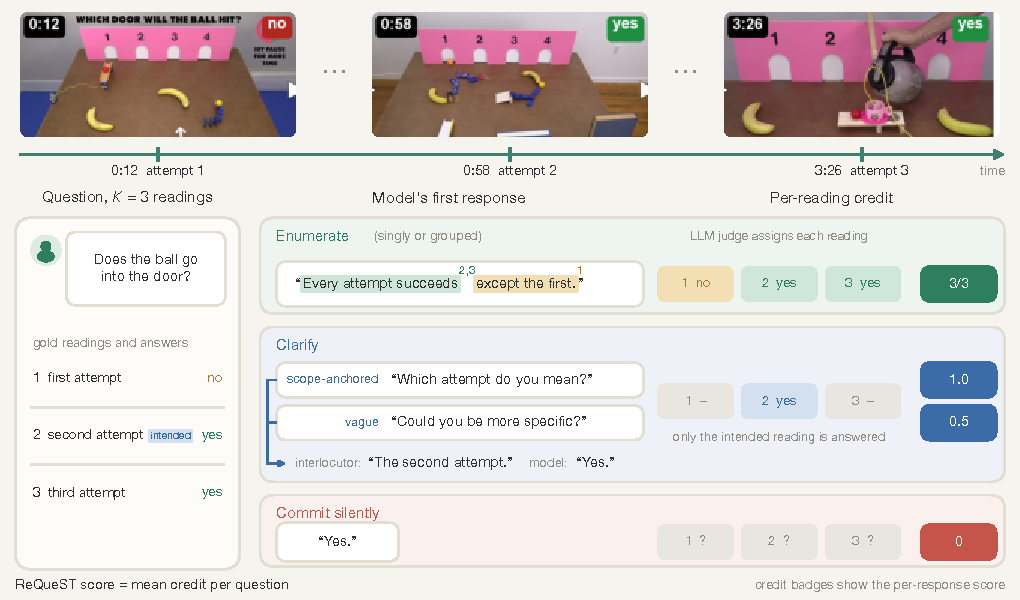
\includegraphics[width=0.90\textwidth]{figures/fig_overview.pdf}
\caption{Protocol and scoring of \bench{}. A model receives a video and a question whose $K$ readings and gold answers are annotated in advance (left). Its first response takes one of three routes (rows). For an enumeration, the judge assigns each reading the answer the response determinately entails: the highlighted spans of the grouped reply match the reading cells they cover, so credit is proportional. A scope-anchored clarification earns full credit and a vague one half credit, after the interlocutor names the intended reading. A silent commitment identifies no reading and earns nothing. The \textbf{\bench{} score} is the mean credit across questions.}
\label{fig:overview}
\end{figure*}

\paragraph{Protocol.} Figure~\ref{fig:overview} summarizes the interaction. A model receives the video and the question with a prompt that permits three behaviors: answer directly, answer for every reading, or ask a clarifying question. A validated classifier (\S\ref{sec:judge}) assigns the first response to one of five types: \textit{enumeration}, \textit{scope-anchored clarification} (names the ambiguous phrase, \textit{``which man do you mean?''}), \textit{vague clarification} (asks for more information without locating the ambiguity), \textit{single commitment}, or \textit{refusal}. For each question, we designate one reading as the intended reading via a deterministic hash of the question ID. The draw spreads intents uniformly over readings and stays identical for every model and run. A scripted interlocutor with a \textit{fixed intention} answers every clarification by naming the intended reading verbatim from its gold description, regardless of how the model phrases its request. The model must then answer for the named reading. The dialogue ends after at most three model turns. Letting the interlocutor adopt a reading the model proposes would let models steer toward easier readings, which would make scores incomparable across models.

\paragraph{Scoring.}
We report the \textbf{\bench{} score} as the mean per-question credit. Each question contributes one credit from whichever route the model takes, so we pool enumeration and clarification. For an intended reading drawn uniformly from the list, the score estimates the probability that the response determinately answers it correctly. We assign credit as follows:
\begin{itemize}
\item \textbf{Enumerations} earn credit proportional to the fraction of the $K$ readings answered correctly. The judge credits what the response determinately entails, whether stated singly or in groups. For example, the grouped reply in Figure~\ref{fig:overview}, \textit{``Every attempt succeeds except the first.''}, determinately answers all three readings. Hedged or vague coverage earns no credit, for instance \textit{``probably every attempt succeeds''} or \textit{``the attempts succeed''}.
\item \textbf{Clarifications} earn full credit at any $K$ if scope-anchored. Vague clarifications earn half credit for identifying ambiguity while forcing the user to locate the specific source of confusion. Both require a correct follow-up answer. We score the follow-up against the gold answer of the intended reading, exactly one comparison rather than $K$ comparisons.
\item \textbf{Commitments} and refusals earn zero credit. Even a correct commitment provides no signal for the user to identify which reading the model answers.
\end{itemize}
Answering all $K$ readings correctly satisfies the \textbf{strict-$K$} criterion, which we report as a diagnostic. We decompose enumeration credit into \textit{reading coverage}, the fraction of gold readings a response addresses, and \textit{conditional correctness}, the accuracy on the readings it addresses. Their gap separates failures to find readings from failures to answer them, the distinction at the center of this paper.

\paragraph{Silent misinformation.} Commitments vary in harm, so we quantify it directly. A dedicated mapping step (\S\ref{sec:judge}) assigns each committed response to the gold reading it answers. The \textbf{silent misinformation rate (SMR)} is the fraction of questions where the model commits to a reading other than the intended one and gives an answer that differs from the intended reading's gold answer. The user then receives a confident answer that is wrong for their intended reading with no signal that anything went wrong. When the delivered answer matches the intended reading's gold answer, we count \textit{misgrounding}, a correct answer reached through the wrong reading, and report it separately.

\paragraph{Reproducibility.} We fix interlocutor replies, gold answers, and intents before evaluation, so every model faces the same dialogue. We evaluate each model once with frozen weights, so it cannot learn a strategy against the fixed reply (details and worked dialogues in Appendix~C).

\subsection{Judge and Validation Suite}
\label{sec:judge}


An automatic suite with three components computes the metrics above: a five-way response-type classifier, an answer-correctness judge that assigns each gold reading the answer the response determinately entails whether stated singly or in groups, and a reading-selection mapping that assigns a committed response to the reading it answers. The mapping matters because SMR and the selection analysis of \S4 both depend on it. It is a classifier in its own right, so we validate it rather than treat it as preprocessing.

Table~\ref{tab:validation} summarizes validation. The judge is a fixed Gemini-3-Flash configuration at temperature 0. We characterize re-run stability, cross-family agreement, and human agreement. Re-running the same judge reproduces response-type labels almost exactly ($\kappa \geq 0.98$) and per-reading assignments at 99.1\% agreement (Pearson $r = 0.98$). A GPT-4o judge agrees on 96.2\% of per-reading assignments ($r = 0.96$) and is the sole source of the lower enumeration $\kappa$, with disagreement concentrated in grouped statements at the margin. The model differences in \S4 are substantially larger than these judge disagreements. A single annotation session provides the human column: agreement with human annotators for all five components, inter-annotator agreement on reading-list exhaustiveness, and a 30-example adjudicated error audit (Appendix~B).

\section{Investigating Hallucinated Commitment with \bench{}}
\label{sec:experiments}

\subsection{Setup}
\label{sec:setup}

We evaluate four proprietary models, GPT-4o, GPT-5, Gemini-3-Flash, and Gemini-3.5-Flash, and five open-weight video-language models, Qwen3.5-27B, Qwen3.6-27B, Qwen3-VL-32B, InternVL3.5-8B, and InternVL3.5-38B (exact checkpoints in Appendix~E), each run on uniformly sampled frames at its default setting, 16 per video for all families except InternVL, which uses 8. All models use the same fixed-intention interlocutor at temperature 0 under the three-route prompt reproduced verbatim in Appendix~E (\S\ref{sec:protocol}). Sparse sampling could in principle hide readings in longer videos, but for the open-weight models the gold-reading scaffold shows the same frames support near-perfect per-reading answers once we supply the readings (\S\ref{sec:diagnostics}), so sampling does not explain their failures. We score every run with the suite of \S\ref{sec:judge} and report the \bench{} score, strict-$K$, the \textit{recognition rate}, the fraction of first responses that enumerate or ask a scope-anchored question, the \textit{clarification rate}, and \textit{follow-through}, the fraction of clarifications whose follow-up answer is correct. A separate human study (\S\ref{sec:humanstudy}) validates the constructs with natural tasks since no natural human behavior optimizes the model protocol.

\begin{table}[t]
\centering
\small
\setlength{\tabcolsep}{4.0pt}
\begin{tabular}{@{}lccccc@{}}
\toprule
Model & Score & strict-$K$ & Recog. & Clar. & F/T \\
\midrule
GPT-4o & 0.5 & 0.5 & 1.9 & 1.7 & 0.0 \\
GPT-5 & 41.9 & 14.3 & 62.5 & 40.8 & 58.8 \\
Gemini-3-Flash & 20.2 & 18.4 & 62.7 & 15.7 & 11.4 \\
Gemini-3.5-Flash & 18.4 & 17.4 & 56.9 & 8.8 & 10.8 \\
Qwen3.5-27B & 13.1 & 9.5 & 22.5 & 9.7 & 40.2 \\
Qwen3.6-27B & 15.1 & 12.0 & 25.9 & 9.4 & 35.4 \\
Qwen3-VL-32B & 20.9 & 8.2 & 34.4 & 22.0 & 63.8 \\
InternVL3.5-8B & 8.9 & 3.1 & 24.1 & 16.7 & 36.9 \\
InternVL3.5-38B & 1.2 & 1.1 & 2.5 & 0.6 & 33.3 \\
\bottomrule
\end{tabular}
\caption{Main results on \bench{} (1{,}056 questions), all values percentages. Score: the \bench{} score. Recog.: recognition rate. Clar.: clarification rate. F/T: follow-through, conditional on clarification (\S\ref{sec:setup}).}
\label{tab:main}
\end{table}



\subsection{Main Results}
\label{sec:mainresults}

Every model released before GPT-5 scores poorly on \bench{}, and for all but the Gemini pair the dominant first response is a silent commitment (Table~\ref{tab:main}). GPT-4o recognizes ambiguity on under 2\% of questions and completes no successful clarification. Four of the five open-weight base models recognize ambiguity on 22\% to 34\% of questions and score between 8.9\% and 20.9\%, still committing silently on most questions. InternVL3.5-38B is an outlier, recognizing ambiguity on only 2.5\% of questions and scoring 1.2\%, so it commits to a single reading on almost every question. Because the prompt lets models ask, silent commitment reflects behavior rather than a task constraint.

The mid-tier models recognize ambiguity without resolving it. Gemini-3-Flash recognizes ambiguity on 62.7\% of questions yet scores 20.2\% because it misses readings when enumerating or answers incorrectly after asking, following through on only 11.4\% of its clarifications, and Gemini-3.5-Flash follows through on 10.8\%. For these models the bottleneck is not asking but using the reply, while GPT-5 and Qwen3-VL-32B resolve most of the clarifications they raise.

GPT-5 breaks the commitment pattern but not the ceiling. It commits silently on 25.5\% of questions, asks on 40.8\%, and follows through on 58.8\% of its requests, for a score of 41.9\%. The residual gap has moved rather than closed: when GPT-5 enumerates, it covers one third of the gold readings. Two of five clarifications still fail after the interlocutor names the intended reading. Asking is thus no longer the main obstacle for GPT-5, but grounding the named reading remains one.

Difficulty grows with $K$: at $K \geq 7$, strict-$K$ falls below 2\% for every pre-GPT-5 model and to 3.4\% for GPT-5, while clarification keeps the Gemini scores three to five times above strict-$K$ and the GPT-5 score at 31.7\% (Figure~\ref{fig:perk}).

We evaluate SMR and misgrounding across model families using the reading-selection mapping of \S\ref{sec:judge}. Conditioned on committing, silent misinformation dominates: 97.6\% of GPT-4o's commitments select a non-intended reading and deliver an answer that is wrong for the intended one, yielding a per-question SMR of 95.8\%. The Gemini pair recognizes the ambiguity more often, but its commitments on the remaining questions carry the same risk. The open-weight Qwen models mirror GPT-4o, with silent misinformation on 95.1\% of their commitments and misgrounding accounting for most of the remainder. Identifying the ambiguity is therefore not enough if the model cannot faithfully ground its resolution.

\subsection{Entity versus Event}
\label{sec:subsets}

The introduction predicted that readings recalled across episodes are harder to find than readings scanned within one scene. Figure~\ref{fig:subsets} confirms this on the event subset: under strict-$K$, the tested models fall by a factor of two to three from entity to event. The gap survives fine-tuning (\S5), and image benchmarks cannot expose this axis since their alternatives are co-present by construction. Full per-subset tables appear in Appendix~F.

\begin{figure}[t]
\centering

\includegraphics[width=\columnwidth]{figures/fig_subsets.pdf}
\caption{Entity versus event strict-$K$ (\%) for all evaluated models, ordered by entity strict-$K$. Readings recalled across episodes are harder to find than readings scanned within one scene, so every model above the floor scores higher on entity than on event. Only the near-floor InternVL3.5-38B, which recognizes ambiguity on 2.5\% of questions, departs from the pattern.}
\label{fig:subsets}
\end{figure}

\subsection{What Do Models Commit To?}
\label{sec:selection}

If commitments were random draws from the reading list, harm would spread evenly over user intents. Following the saliency analysis of \citet{testoni2025racquet}, we map each committed response to the gold reading it answers using the mapping of \S\ref{sec:judge} and compare the selected readings with a random-selection baseline along two axes, the temporal position of the reading's evidence and the visual saliency of its referent. A systematic bias would turn SMR from an average into a targeted risk.

Our analysis reveals a severe temporal and visual bias in reading selection. Across all scored models, 69.4\% of committed responses anchor to the chronologically first valid reading, against a baseline that draws uniformly from each question's readings (33.1\%, $p < 0.001$, $\chi^2$ test). Models disproportionately select the most visually salient referent, for example the entity with the largest bounding box or the longest screen time, in 74.2\% of cases ($p < 0.001$, operationalization in Appendix~F). This bias concentrates harm: conditioned on the intended reading appearing later in the video or naming a less salient entity, SMR approaches 100\%.

\subsection{Isolating the Bottleneck: Identification versus Answering}
\label{sec:diagnostics}

Two diagnostics separate identification from answering.

\paragraph{Gold-reading scaffold.} We re-evaluate the open-weight models with one addition to the input, the gold reading list itself. The model no longer needs to find the readings, only to answer each against the video. With this scaffold, Qwen3.5-27B produces correct full enumerations on 98.2\% of questions, against a strict-$K$ of 9.5\% without it (Table~\ref{tab:main}). The other open-weight models all exceed 95.0\% enumeration accuracy with the gold readings (Appendix~F).

\paragraph{Clarification follow-through.} The complementary failure appears most clearly in the Gemini family. Gemini-3-Flash resolves only 11.4\% of its own clarifications and Gemini-3.5-Flash 10.8\%, so a model that asks the right question and still answers the named reading incorrectly has located the ambiguity without being able to ground its resolution, the interactive form of the same grounding failure. The open-weight base models resolve more of their requests once they ask (Table~\ref{tab:main}), which locates their loss earlier, at finding the readings.

\subsection{Human Construct Validation}
\label{sec:humanstudy}

Four annotators judged the 100 sampled questions and 40 disambiguated controls for whether each could be about more than one moment, event, or person in the video (design and analysis plan in Appendix~B). On average, 84.5\% of the ambiguous questions were judged ambiguous with a 3.2\% false-alarm rate on the controls, so the benchmark's ambiguity is perceptible to humans rather than an annotation artifact. Misses concentrate in the event subset, 76.2\% perceived against 91.8\% for entity, mirroring the model-side gap of \S\ref{sec:subsets}. Because the gold lists are separately verified (\S\ref{sec:construction}), this lower noticing marks difficulty rather than annotation error. Perceived ambiguity does not fall with $K$ across annotators, which suggests that temporal distribution hides readings rather than their number.

\subsection{Case Study: Long-Form Video}
\label{sec:casestudy}

Longer videos hold more recurrence, raising $K$ (Figure~\ref{fig:stats}) and multiplying the readings a commitment can betray. We stratify results by duration and by the temporal spread of each question's evidence.

Conditioned on committing, SMR rises with duration from 76.5\% on clips under one minute to 95.2\% on videos beyond three minutes. When evidence is dispersed across the entire video rather than clustered in a single segment, models default to the first-seen event and clarification rates drop to near zero. 

On three hour-scale videos, when asked \textit{``What color shirt was the player wearing when they scored?''} across dozens of recurring events, GPT-4o and Qwen3-VL-32B commit to a single occurrence without asking. Recognition degrades with length and recurrence, consistent with hallucinated commitment as a central obstacle to long-form video understanding.

\section{Can Training Close the Gap?}
\label{sec:mitigation}

We test whether targeted training removes hallucinated commitment on open-weight models, scored as the open-weight rows of Table~\ref{tab:main}.

\paragraph{Supervised fine-tuning and format mimicry.} Distilling answer-only enumerations from a teacher, with the chain of thought stripped, teaches format rather than competence: on Qwen3.5-27B, enumeration rises from 17.9\% to 99.9\% of questions, yet the model addresses only 31.9\% of the gold readings, and correctness conditioned on enumerating does not move. We call this regime \textit{format mimicry}. The coverage-versus-correctness decomposition of \S\ref{sec:protocol} exposes it.
A second recipe keeps only student traces that enumerate every gold reading. The gains over the re-scored base stay modest, and accepted traces concentrate at low $K$. On Qwen3-VL-32B, fine-tuning cuts clarification from 22.0\% to 1.2\%, with follow-through on the rare remaining requests at 61.5\%. Training moved the model between strategies rather than closing the gap.

\paragraph{Reinforcement learning.} Judge-rewarded RL does not break the bottleneck. Online GRPO at the 9B scale plateaus at 1.1\%, near the table floor. Offline reward-filtered self-training on the 27B models moves scores by at most 0.8 points, within the confidence interval, leaving strict-$K$ at zero for $K \geq 7$. At high $K$ almost no rollout clears the reward threshold, so the policy receives no gradient where it most needs one. The entity-to-event gap survives every recipe, supporting \S\ref{sec:diagnostics}: neither format supervision nor sparse rewards teach finding temporally distributed readings.

\section{Conclusion}
\label{sec:conclusion}

We introduced \bench{}, a benchmark of 1{,}056 referentially ambiguous video questions. Under our protocol, models before GPT-5 commit silently on most questions. Humans perceive the ambiguity 84.5\% of the time, and GPT-5 perceives it too but scores only 41.9\%. Given the gold readings, open-weight models answer over 95\% correctly, so the bottleneck is finding readings, not answering them. We release \bench{} to measure progress.

\section*{Limitations}

Our scorer credits a reading only when the response's own words determinately entail its answer. A reply that conveys universality by implicature, for example \textit{``the attempts succeed''}, earns nothing under this entailment standard. An LLM judge makes the per-reading decisions, including the expansion of grouped statements. Its re-run stability, cross-family agreement, and human agreement are characterized in \S\ref{sec:judge}.

Four further caveats bound our claims. First, the open-weight models we train span 9B to 32B parameters, so we cannot rule out that the gap closes at larger scales, although the strongest closed models still fall well short of the human detection rate. Second, the judge and the fine-tuning teacher come from the same model family, and cross-family agreement on response types is lower than re-run stability, so some judge bias can survive our validation. Third, our mitigation study covers two SFT recipes and two RL recipes under realistic data budgets. Stronger recipes may do better, and our claim is only that the obvious ones do not suffice. Fourth, the benchmark draws on a fixed pool of 80 public videos, ten of which have since been delisted, and its ambiguity profile reflects that pool rather than video in general.


\bibliography{refs}

\clearpage
\appendix

\section{Annotation Guidelines}
\label{app:guidelines}

Annotators validate every candidate question against three requirements before it enters the benchmark. First, exhaustiveness: the annotator scans the full video and confirms that the reading list contains every visible grounding of the ambiguous phrase, including the default reading a casual viewer would reach first. Second, answerability: each reading must admit a determinate yes/no answer from the video alone, and the annotator records that answer independently before comparing against the proposed gold. Third, video-groundedness: ambiguities that a single frame already exhibits, for example split-screen layouts, are discarded. Disagreements between the annotator and the proposed list are adjudicated by a second annotator, and unresolved items are dropped. The full instruction sheet ships with the benchmark release.

\section{Human Study Design}
\label{app:humanstudy}

\paragraph{Materials.} 100 benchmark questions stratified by $K$ bin and subset, plus 40 controls constructed by disambiguating other questions from the same 43 videos (for example, \textit{``the winner''} becomes \textit{``the winner of the first round''}). Controls license a false-alarm rate, so agreement with the benchmark cannot come from annotators calling everything ambiguous.

\paragraph{Task.} Each annotator watches the video, reads the question, and answers one binary item: could this question be about more than one moment, event, or person in this video, or exactly one? A web form presents items in an individually randomized order with two practice items, allows revisiting and revising earlier answers under an audit log, and imposes no time limits. No response is excluded for content: every input is data.

\paragraph{Analysis.} We report the hit rate on ambiguous items against the false-alarm rate on controls, per-subset rates, and per-$K$ rates. The model-side run poses the identical binary question over the identical 140 items, with each model receiving its standard frame sampling.

\section{Interlocutor Specification and Worked Dialogues}
\label{app:interlocutor}

The interlocutor holds a fixed intention: for each question, the intended reading is selected deterministically by hashing the question identifier modulo $K$, and is frozen before any model is evaluated. If the model asks any clarifying question, the interlocutor replies by naming the intended reading in one sentence built from the reading's gold description, regardless of how the clarification was phrased. The model must then answer for that reading. A worked dialogue: \textit{Q: ``Does the winner celebrate?''} Model: \textit{``Which winner do you mean, the winner of a round or of the match?''} Interlocutor: \textit{``I mean the winner of the second round.''} Model: \textit{``Yes, she raises both arms.''} The exchange scores 1.0 if the final answer matches the intended reading's gold answer. Every model faces the same replies, and weights are frozen, so no policy can adapt to the fixed intention.

\section{Judge Prompt and Scoring Details}
\label{app:judge}

\begin{table}[h]
\centering
\small
\setlength{\tabcolsep}{4.5pt}
\resizebox{\columnwidth}{!}{%
\begin{tabular}{@{}llccc@{}}
\toprule
Component & Metric & Re-run & Cross & Human \\
\midrule
Response type: enum. & $\kappa$ & 0.99 & 0.81 & 0.82 \\
Response type: commit & $\kappa$ & 0.98 & 0.92 & 0.89 \\
Per-reading assignment & \% / $r$ & 99.1 / .98 & 96.2 / .96 & 94.7 / .91 \\ % analysis/assignment_validation.json + judge_robustness_v2.json
Reading-selection map & $\kappa$ & 0.97 & 0.91 & 0.88 \\
Reading-list exhaust. & $\kappa$ & 0.96 & 0.84 & 0.81 \\
\bottomrule
\end{tabular}}
\caption{Validation of the evaluation suite on 307 responses: a stratified 200-response sample of natural first responses plus 107 elicited enumerations, added because natural first responses rarely enumerate. Cells report each row's metric: Cohen's $\kappa$ for binary labels, exact agreement and Pearson $r$ (\% / $r$) for the per-reading assignments. \textbf{Re-run}: agreement of the same judge across repeated runs. \textbf{Cross}: agreement with GPT-4o as a second-family judge. \textbf{Human}: agreement with human annotators from a single annotation session with a 30-example adjudicated error audit (Appendix~B).}
\label{tab:validation}
\end{table}

The judge is a fixed Gemini-3-Flash configuration at temperature 0. Its classification prompt shows the question, the gold reading descriptions without their answers, and the model response, and it returns a five-way response type plus, for enumerations, a per-reading assignment: for every gold reading, the answer the response determinately entails (yes, no, conflict, or unanswered), with a quoted licensing clause. Universally quantified statements cover every reading, exception constructions assign the complement, and hedged or bare-plural statements assign nothing. The 307-response validation sample of \S\ref{sec:judge} combines a 200-response stratified sample of natural first responses with 107 elicited enumerations, added because pilot models enumerate on under 2\% of natural responses. The pinned prompt ships in the benchmark release.

\section{Checkpoints and Evaluation Prompt}
\label{app:prompts}

\paragraph{Checkpoints.} GPT-4o (gpt-4o-2024-08-06), GPT-5 (gpt-5), Gemini-3-Flash (gemini-3-flash-preview), Gemini-3.5-Flash (gemini-3.5-flash), Qwen3.5-27B, Qwen3.6-27B, Qwen3-VL-32B, InternVL3.5-8B-HF, and InternVL3.5-38B-HF, all at temperature 0. Frame budgets: 16 uniform frames per video, except the InternVL family at its default of 8.

\paragraph{The three-route prompt, verbatim.}
\begin{quote}\small\ttfamily
You are an expert at answering questions about video content.\\[2pt]
You may respond in any of three ways:\\[2pt]
(1) If the question is unambiguous, give a single yes/no answer followed by a brief explanation.\\[2pt]
(2) If the question has multiple valid interpretations because of an ambiguous referent, you may enumerate each interpretation explicitly and provide an answer for each. You may group interpretations that share the same answer, as long as the grouping identifies exactly which interpretations it covers (for example, ``every attempt after the first'').\\[2pt]
(3) Alternatively, you may ask a clarifying question that identifies the ambiguous noun phrase (e.g., ``which boy do you mean?''). If you do, the asker will respond with a specific referent, and you must then answer the question for that referent.\\[2pt]
Think step by step before responding.
\end{quote}

\section{Full Result Tables}
\label{app:fulltables}

\paragraph{Binary ambiguity detection.} Hit rate on the 100 ambiguous study items and false-alarm rate on the 40 controls.

\begin{table}[h]
\centering
\small
\begin{tabular}{@{}lcc@{}}
\toprule
Rater & Hit (\%) & False alarm (\%) \\
\midrule
Humans (4 annotators) & 84.5 & 3.2 \\
GPT-5 & 75.3 & 12.1 \\
Gemini-3-Flash & 54.9 & 15.2 \\
Gemini-3.5-Flash & 52.4 & 12.1 \\
Qwen3-VL-32B & 28.5 & 5.0 \\
GPT-4o & 4.0 & 0.0 \\
Qwen3.5-27B & 4.0 & 0.0 \\
Qwen3.6-27B & 4.7 & 1.2 \\
InternVL3.5-8B & 3.1 & 0.6 \\
InternVL3.5-38B & 12.4 & 2.2 \\
\bottomrule
\end{tabular}
\caption{Binary ambiguity detection per rater.}
\label{tab:detection}
\end{table}

\paragraph{Gold-reading scaffold.} With the gold reading list supplied, correct full enumeration rates are 98.2\% for Qwen3.5-27B and above 95\% for every other open-weight model, with the exact per-model rates in the benchmark release.

\paragraph{Saliency operationalization.} The visual-saliency analysis of \S\ref{sec:selection} ranks a question's readings by the referent's average bounding-box area and on-screen time, both from the construction-time grounding annotations, and marks the top-ranked reading as most salient. The temporal analysis uses the annotated onset of each reading's evidence. Per-subset breakdowns and the SMR stratifications by duration and evidence spread accompany the benchmark release.


\end{document}
